% Chapter 6

\chapter{Conclusions} % Main chapter title

\begin{figure}[hbtp]

\centering
    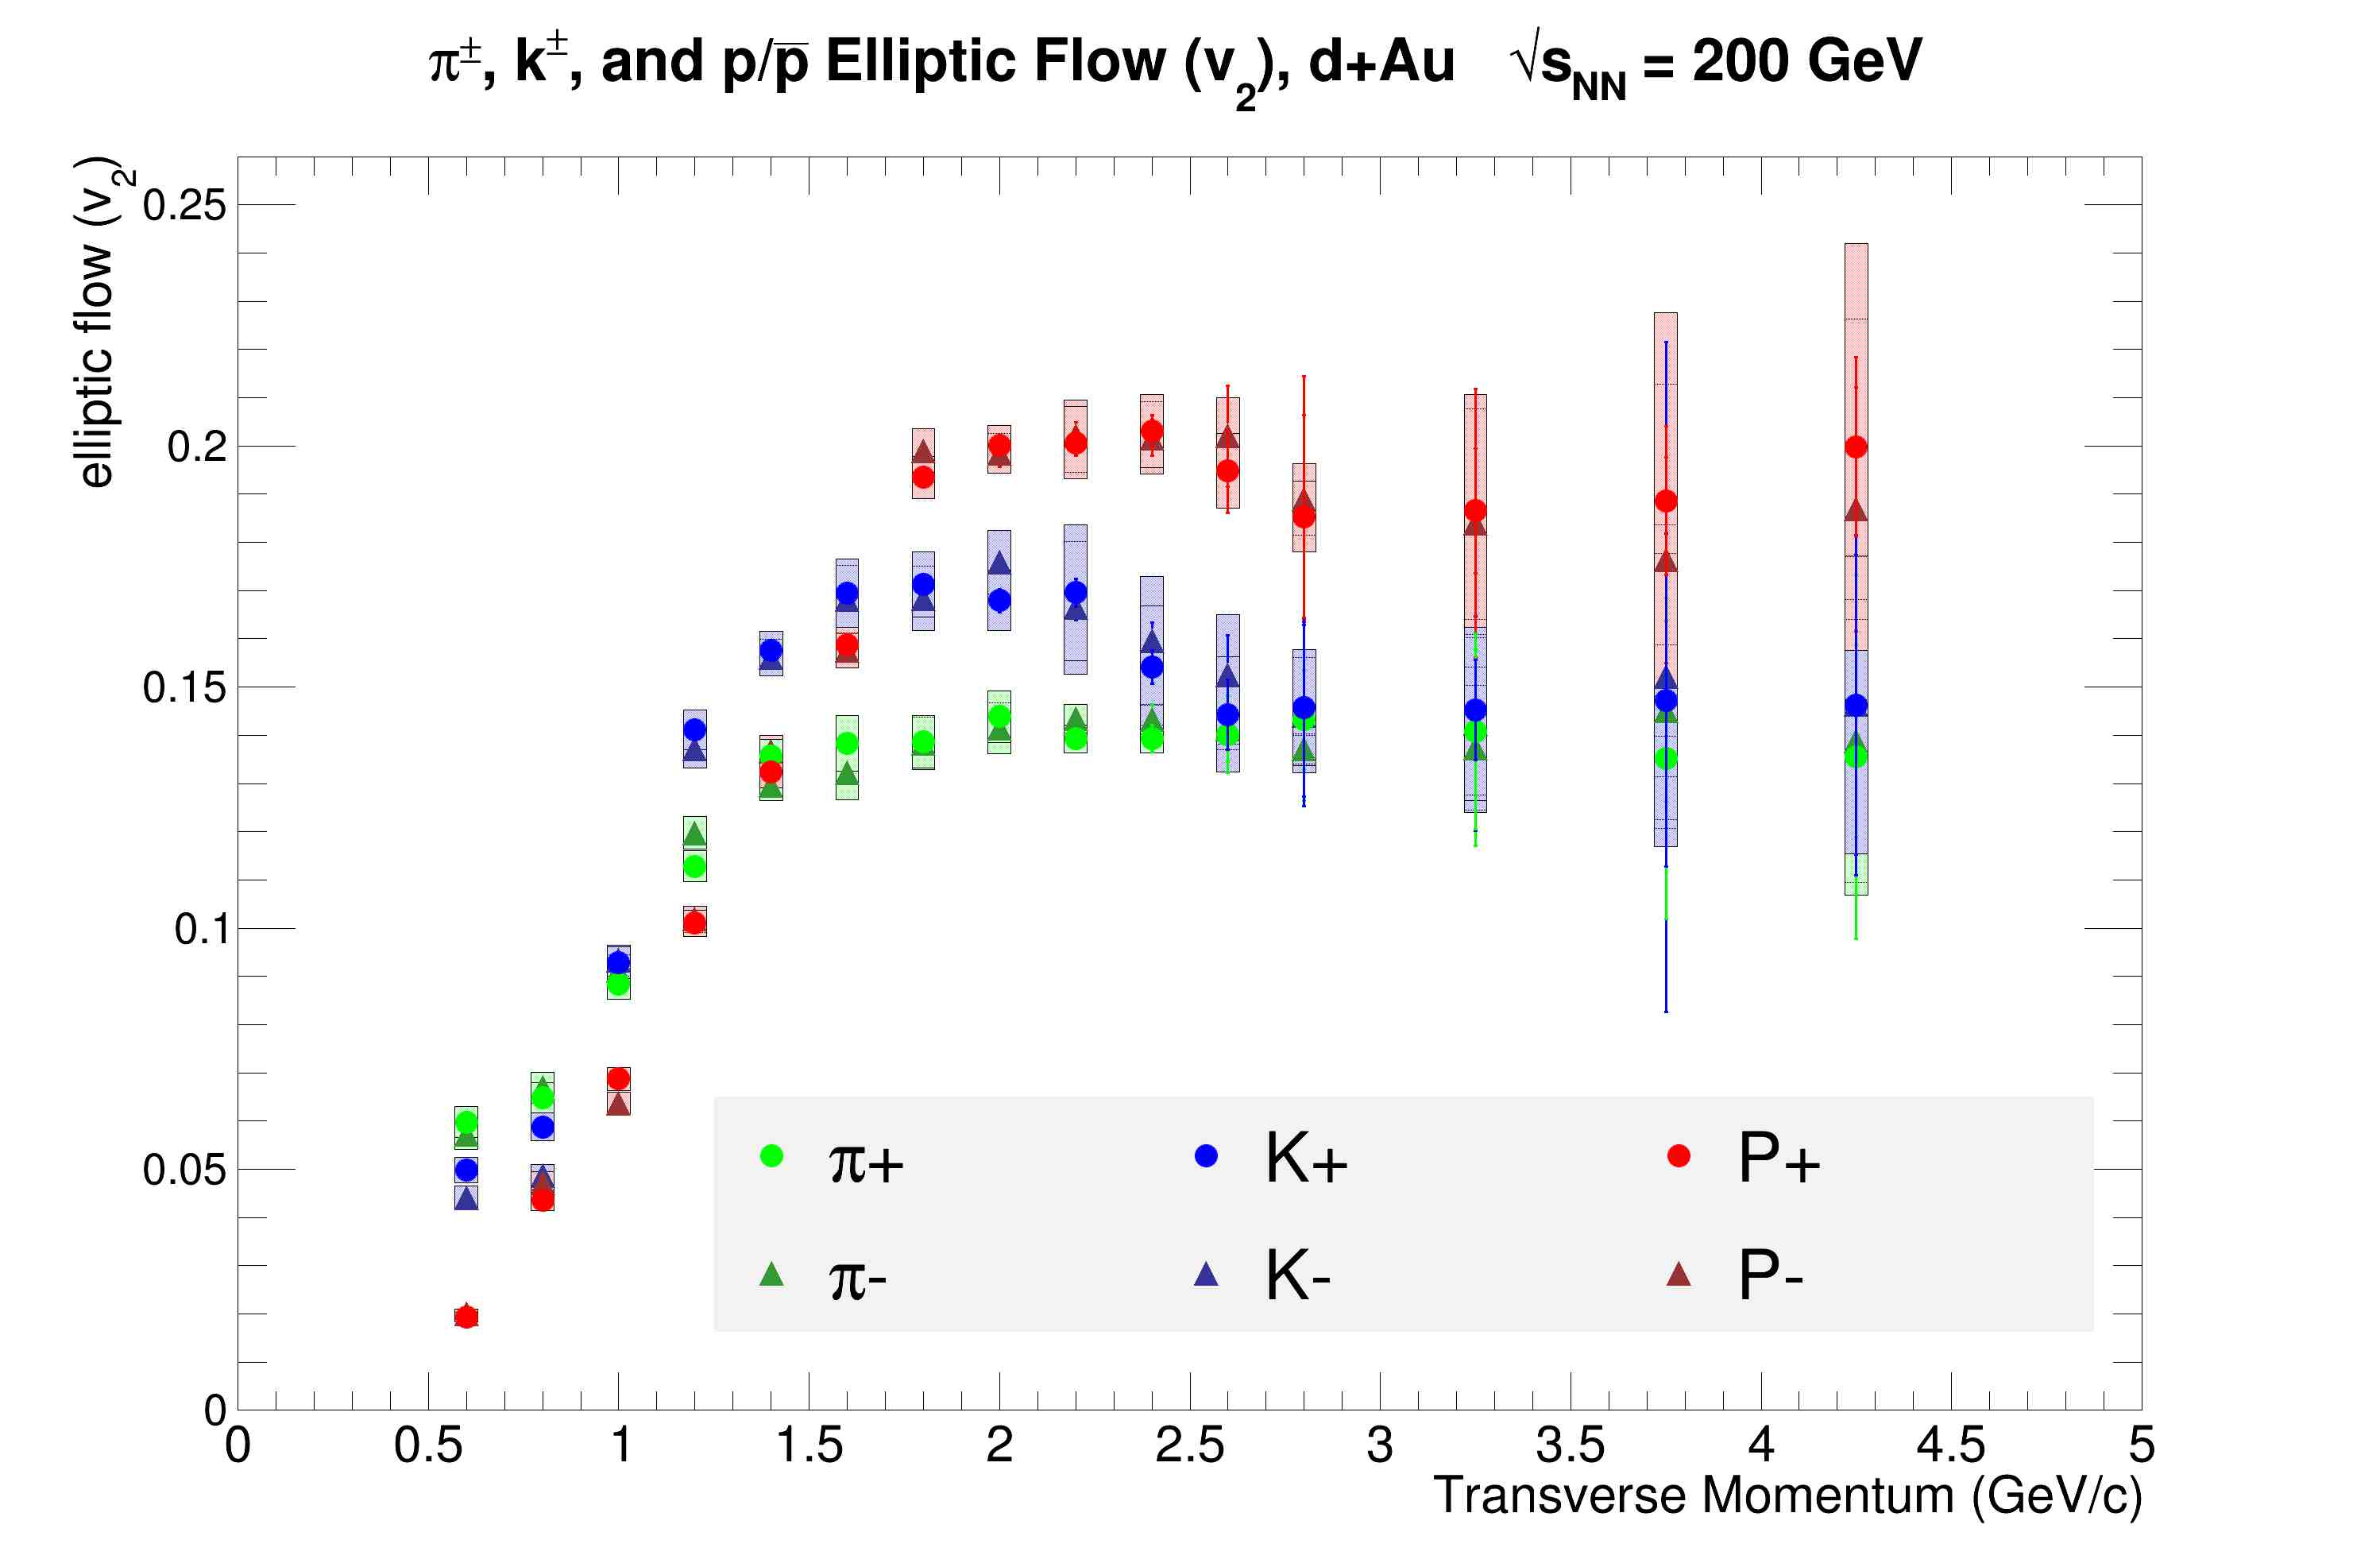
\includegraphics[width=0.7\textwidth]{results/v2all.jpg}
    \rule{35em}{0.5pt}
    \caption[Elliptic Flow vs Transverse Momentum, 200 GeV d+Au]{Elliptic Flow vs Transverse Momentum, 200 GeV d+Au}
    \label{fig:v2main}
\end{figure}

Measurements of the second Fourier coefficient corresponding to an elliptically shaped azimuthal anisotropy of pions, kaons, and (anti)protons produced in 200 GeV deuteron-gold collisions are presented in figure \ref{fig:v2main}. This measurement is a sign that collective behavior happens in systems previously thought of as ``cold'' and is an indication that a QGP could be formed in the simpler system of d+Au. This flow increases steadily for all hadrons up to $p_T \sim 1.5 $ GeV/c where the mesons (pions and kaons) seem to reach a saturation and flatten out. The kaons exhibit a flow signal stronger than the pions in this range but eventually decreasing to the same nominal value as the pions. The (anti)protons continue to flow increasingly up to $p_T \sim 2$ GeV/c. 

\section{Discussion}

\subsection{Hadronization}
\begin{figure}[hbtp]
\centering    
    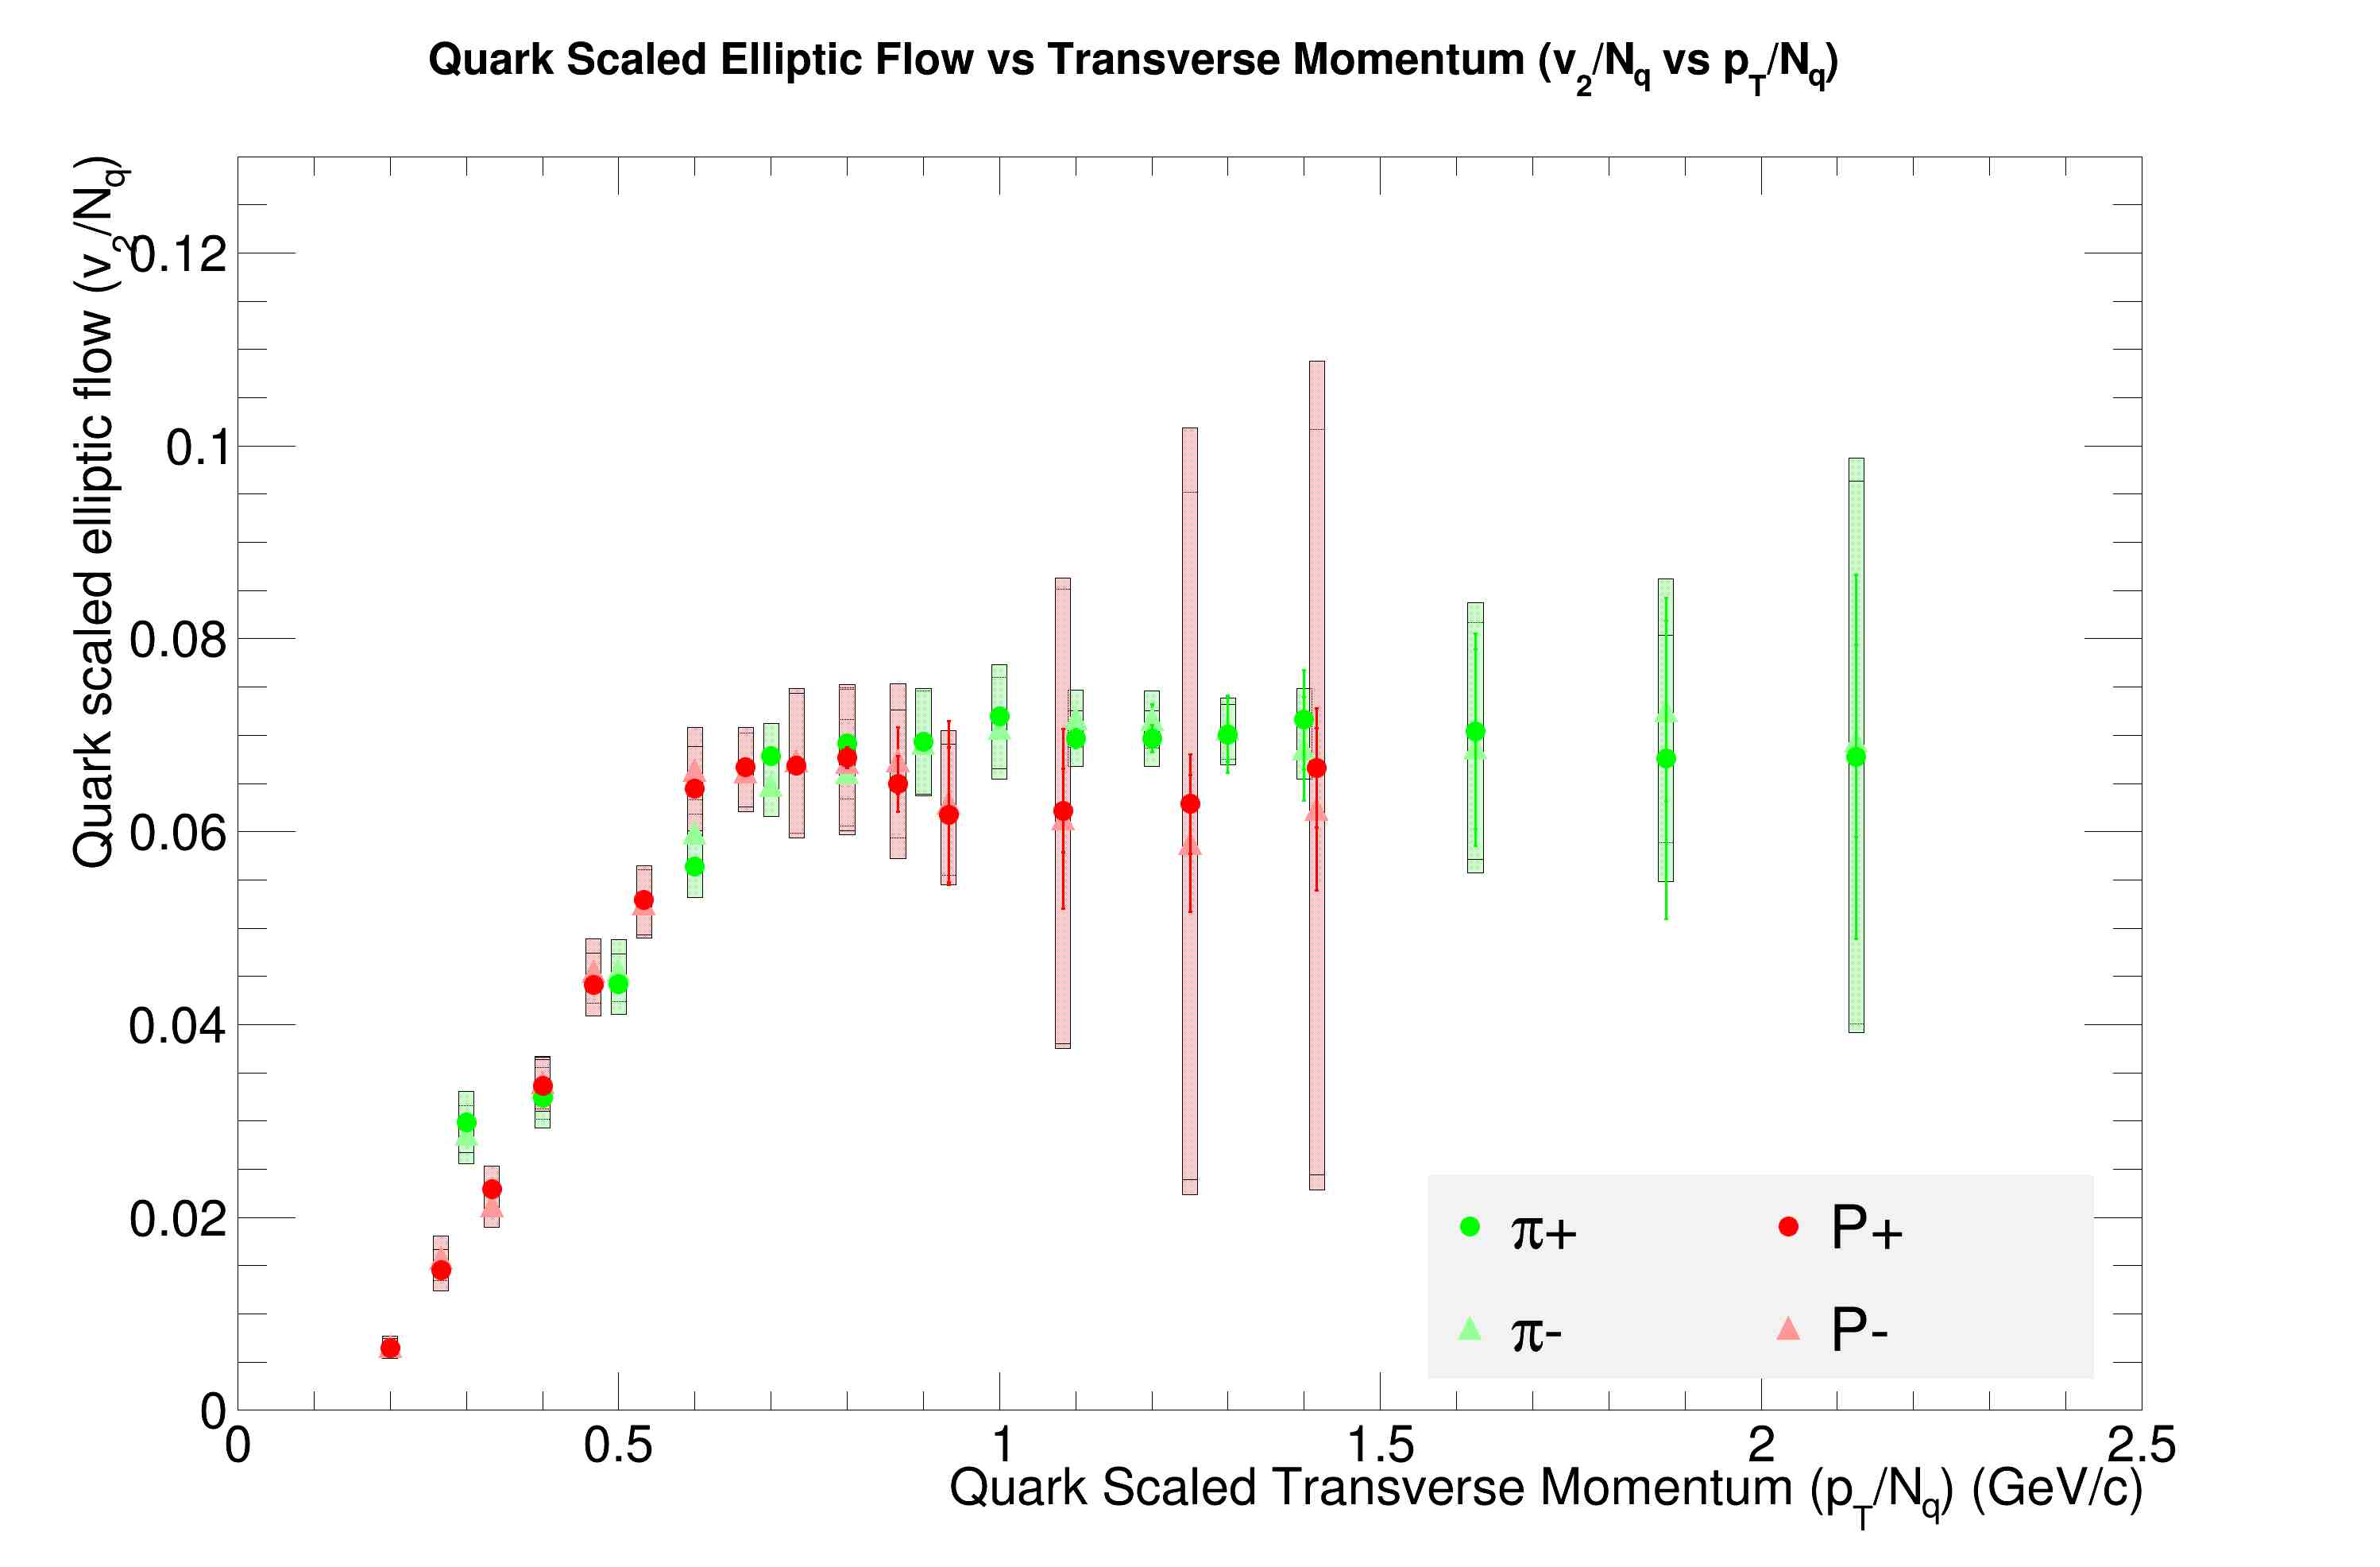
\includegraphics[width=0.7\textwidth]{results/v2NqvspT.jpg}
    \rule{35em}{0.5pt}
    \caption[Quark Scaled Elliptic Flow ($\pi^{\pm}$ and $p/\bar{p}$) vs Transverse Momentum, 200 GeV d+Au]{Quark Scaled Elliptic Flow ($\pi^{\pm}$ and $p/\bar{p}$) vs Transverse Momentum, 200 GeV d+Au}
    \label{fig:qscaledv2}
\end{figure}

This (anti)proton flow enhancement in the mid-$p_T$ range is indicative of baryon enhancement seen in previous experiments. This enhancement happens in the freeze out stage and may be attributed to recombination/fragmentation effects. Scaling the flow coefficient and momentum by the number of quarks that comprise the measured particle\footnote{2 quarks for pions/kaons, 3 quarks for protons} shows that this particle momentum discrepancy may come from the sum of momenta of the constituent quarks (see fig \ref{fig:qscaledv2}). That is to say, the reason why protons appear to have stronger flow is simply because they contain more quarks. If three quarks with the same momentum combined to produce one particle that particle would have more momentum than if only two of those quarks had combined, a strong indication of recombination as the mechanism for thermal freeze-out, and a result that agrees with similar quark scaled results in He3+Au, Au+Au, Pb+Pb (needs citations).  
\subsection{Initial Conditions}

\subsection{Equilibrium/Flow}




\pagebreak
\pagebreak


